\section{Introduction}


\paragraph{Scale-aware Hyperparameters.}
A central dogma in empirical deep learning is that performance will steadily improve as training data and parameter count increase \citep{hestness2017deep,kaplan2020scaling, hoffmann2022training}. This paradigm incentivizes practitioners to develop increasingly larger trained models while first conducting experiments at smaller, more economical scales. For such small-scale experimentation to effectively inform larger training runs, it becomes crucial to reason about hyperparameters (HPs) in a scale-aware framework and to analyze the behavior of the \textit{sequence} of progressively scaled-up training runs. 
For example, when scaling the width $n$ of a neural network, we should explicitly conceptualize the learning rate as the product of a scale-independent HP $\eta$ and a scaling factor $n^{-a}$. This scale-aware perspective was initially formalized in the Tensor Program series \citep{yang2021tensor, yang2022tensor, yang2023tensor} for the width-scaling of neural networks, with later extensions to other dimensions such as depth \citep{yang2023depth, bordelon2023depthwise, dey2025don, chizat2025hidden}. It was shown theoretically that the correct scaling for ensuring ``optimal'' training in the infinite-width limit $n\to\infty$ is the \textit{Maximal Update Parameterization} \citep[$\mu$P,][]{yang2021tensor}, and under such scaling the optimal HPs are expected to be asymptotically scale-independent. This property is desirable since the HPs do not explode or vanish with scale and hence can be tuned on a fixed, scale-independent grid.

\paragraph{Fast Transfer.} While existing Tensor Programs theory suggests asymptotic scale independence of hyperparameters, it does not predict how quickly optimal HPs converge with scale. Empirical evidence \citep{yang2022tensor, lingle2024empirical}, however, has demonstrated that $\mu$P exhibits \textit{fast} hyperparameter transfer in practice. Fast HP transfer occurs when optimal HPs converge sufficiently fast with respect to scale (see Section \ref{sec:useful-transfer} for a precise statement), allowing practitioners to tune HPs on smaller proxy models and apply these values to larger-scale training runs with minimal performance loss. Despite its practical utility in drastically reducing HP tuning costs, the underlying mechanisms that enable fast transfer remain poorly understood.


\subsection{Our Contributions}
We provide insight into the puzzle of fast HP transfer by first developing a mathematical framework for reasoning about HP transfer in Section~\ref{sec:framework}. Then in Section~\ref{sec:useful-transfer} we formally define fast HP transfer in terms of convergence rates of optimal HPs and the loss, and provide a direct connection to the ``usefulness'' of transfer when performing compute-optimal grid search. We quantify these convergence rates in synthetic settings, and demonstrate that while valid in certain linear models, fast transfer is not guaranteed in neural networks even when using $\mu$P. Such examples illustrate that the benefits of transfer heavily depend on structural properties of the training process emerging from the data, optimizer, and architecture. 

To illuminate this structure, in Section~\ref{sec:topk_decomposition} we introduce a novel \emph{trajectory decomposition} obtained by decomposing the stepwise linearized loss change along the training trajectory. We empirically demonstrate that the linearization is an effective proxy for the true loss change when considering the \emph{exponential moving average} (EMA) of the optimization trajectory. The faithfulness of this approximation arises due to the smoothness of the resulting EMA trajectory which averages out the oscillations (see Figure \ref{fig:ema_iterate_lin}). 
% We believe that our linearization technique can be powerful tool for studying optimization phenomena more broadly. 
Using this linearization, we track the loss change from the projection of the update in the top-$k$ directions that maximize this change in the loss at each matrix layer of the neural network. This decomposes the total loss change into two components: the \emph{top-$k$ loss} arising from the dominant $k$ components and the remaining \emph{residual loss}. 

\begin{wrapfigure}{r}{0.48\textwidth}  
\vspace{-4mm} 
    \centering
    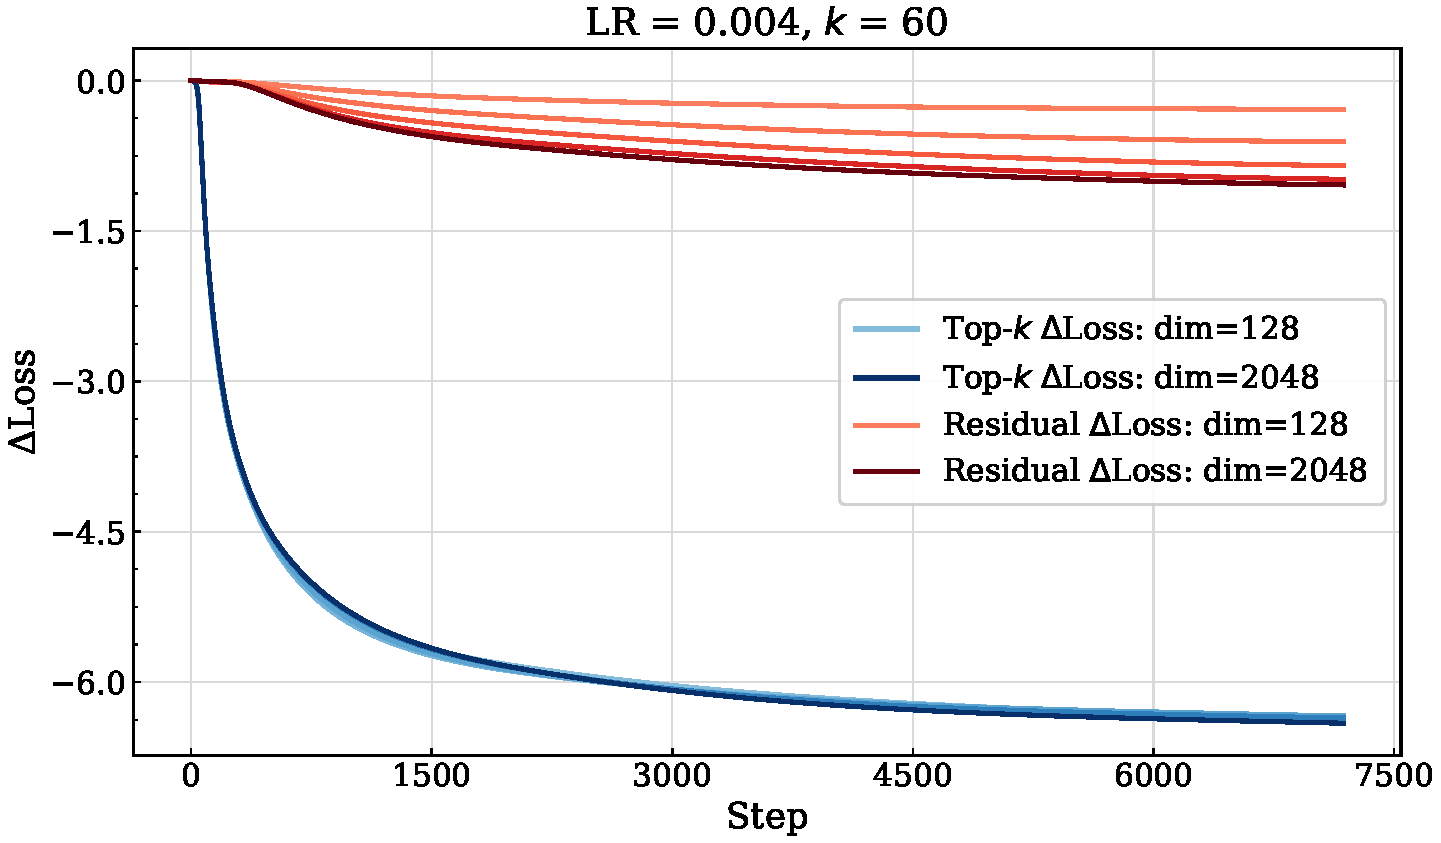
\includegraphics[width=0.48\textwidth,keepaspectratio]{arxiv_figures/split_loss_over_time_lr=0.004_ema=0.9995_seed=0_step_7185.pdf}
    \vspace{-6.6mm}
    \caption{\small Loss decomposition into top-$k$ and residual components in transformers with varying widths.
    }
    \label{fig:split-loss-over-time-step-7185}
    \vspace{-5mm}
\end{wrapfigure}

We conjecture that the training behavior on the top-$k$ subspaces concentrates quickly with width while the remaining directions provide performance gains as the width increases. In Figure~\ref{fig:split-loss-over-time-step-7185} we validate this intuition by applying the loss decomposition introduced in Section~\ref{sec:fast-transfer} to a sequence of Llama-style transformers of increasing width trained under $\mu$P. We observe that the leading top-$k$ loss remains approximately invariant across widths, whereas the residual loss consistently improves with width, especially later in training. Moreover, since the top-$k$ loss provides the majority of the loss decrease, it is reasonable to expect that the optimal learning rate for the total loss will not deviate much from the optimal learning rate for the top-$k$ loss.  

Therefore, for an appropriately chosen $k < n$, the top-$k$ loss decomposition provides the following potential explanation for the phenomenon of fast transfer. 

\refstepcounter{idea}\label{box:fast-transfer}
\begin{tcolorbox}[colback=white, colframe=gray,
  title={Hypothesis~\theidea: Fast Transfer via Loss Decomposition}]
\begin{enumerate}[leftmargin=1em,itemsep=0.2em]
    \item The top-$k$ loss converges rapidly with scale~$n$, hence so do the optimal HPs for the top-$k$ loss.
    \item The optimal HPs for the top-$k$ loss approximately \emph{determine} the optimal HPs for the total loss.
\end{enumerate}
\end{tcolorbox}
We formalize this explanation and introduce an explicit trajectory decomposition (Section~\ref{sec:topk_decomposition}) that separates width-stable and width-sensitive contributions to loss reduction. This decomposition provides the basic lens we use throughout to analyze optimizer dynamics across widths. We use this to demonstrate concretely that Adam and SGD exhibit the high-level structure posited by Hypothesis~\ref{box:fast-transfer}. In Section~\ref{sec:llama_muon}, we apply the same analysis to Muon and obtain a qualitatively different picture: loss reduction is less concentrated in a width-stable top-$k$ subspace and is spread over many directions. This yields a concrete contrast between Adam and Muon dynamics and highlights a potential connection between optimizer geometry and the stability of learning-rate transfer. We further probe this connection via rank-controlled variants to isolate how preconditioning structure modulates the decomposition and transfer. Finally, in Section~\ref{sec:mlp_sgd} we refine the decomposition to operate at the data level, where we observe that width-stable components align with ``easy'' examples and width-sensitive residual directions align with ``hard'' examples in the tail.

\subsection{Related Work}\label{sec:related_work}

\paragraph{Hyperparameter Transfer.}
The concept of HP transfer was introduced by \citet{yang2022tensor}, who showed that HPs tuned on small proxy models can transfer reliably to much larger ones under $\mu$P scaling. Subsequent empirical studies confirmed the effectiveness of learning rate transfer in transformers, while also highlighting certain limitations \citep{lingle2024empirical, vlassis2025thorough}. As \citet{yang2022tensor} noted, the success of HP transfer is not fully explained from first principles. To address this gap \citet{noci2024super} showed empirically that top Hessian eigenvalues converge rapidly under $\mu$P across widths, suggesting a width-stable curvature that could underpin reliable transfer. However, the connection between these spectral statistics and the optimal learning rate remains unclear. More recently, \cite{hong2025provable} established a scale separation between certain macro- and micro-variables, thereby suggesting HPs can be effectively tuned in early training stages. The concurrent work of \cite{hayou2025proof} showed that for linear networks  under $\mu$P, the optimal learning rate admits a nontrivial limit as $n\to\infty$, hence establishing the \textit{weak transfer} condition which we introduce in Section~\ref{sec:framework}; however, as we will see in Section~\ref{sec:useful-transfer}, this condition alone does not imply computational efficiency of HP transfer. In contrast to these results, 
our work introduces a formal framework to reason about when transfer is useful, and explicitly connects the fast convergence of certain statistics of the optimization path (which we define via a trajectory-level loss decomposition) to the fast convergence of optimal HPs. 

\paragraph{Optimization Trajectories.}
Our fast transfer hypothesis rests on the existence of low-dimensional structure in optimization trajectories. \citet{gur2018gradient} observed that gradients rapidly align with top eigenvectors of the Hessian, suggesting that GD operates within a ``tiny subspace.'' \citet{song2024does} refined this view, showing that while gradient variance concentrates in the top eigenspace, motion in these directions primarily drives oscillations rather than loss reduction. This behavior is consistent with edge-of-stability (EoS) \citep{cohen2021gradient,damian2022self} and motivates our use of EMA smoothing: by averaging out oscillatory components tied to the top eigenspace, the smoothed trajectory (analogous to the ``central flow'' \citep{cohen2024understanding}) reveals the low-dimensional subspace where genuine loss decrease occurs. 
Similar low-dimensional structure has also appeared in various theoretical settings on gradient-based feature learning, such as the learning of multi-index models \citep{abbe2022merged,damian2022neural,mousavi2023neural,glasgow2025mean}, where SGD ``localizes'' parameters into low-dimensional subspaces. 
Recent works have also shown that gradient updates induce a spiked (signal-plus-noise) eigenstructure in the conjugate kernel \citep{moniri2023theory,wang2024nonlinear,dandi2024random} or the Hessian \citep{arous2023high,arous2025local,montanari2025phase} of the neural network, and leading eigenvectors contain information of the target function. 
Drawing inspiration from these theoretical works, we explicitly isolate the width-invariant structure in realistic settings using a spectral decomposition and link it to HP transfer.  

\section{Preliminaries and Formal Framework}\label{sec:framework}

We now formalize our framework for HP transfer. We will let $n$ denote the scaling dimension. The scaled HPs used during training at scale $n$ are:
\[
    \scaledhps_n(\bhp, \bhpexp) = (\hp_1 n^{-\hpexp_1}, \ldots, \hp_{\numhps} n^{-\hpexp_{\numhps}}),
\]
where we refer to $\bhp = (\hp_1, \ldots, \hp_{\numhps})$ as the HPs and to $\bhpexp = (\hpexp_1, \ldots, \hpexp_{\numhps})$ as the scaling exponents. Conceptually, $\bhp$ are a set of $n$-independent constants which are tuned for a specific problem and $\bhpexp$ are a set of exponents which specify how to scale the HPs with $n$ so that training can be performed at any scale $n$ using $\scaledhps_n(\bhp, \bhpexp)$. 
In this paper, we focus on the ``optimization hyperparameters'' of the abcd-parameterizations of \citet{yang2023tensor} (see Appendix \ref{app:background}) -- this encompasses the width scaling of HPs needed for training standard neural network architectures using common optimizers such as SGD and Adam.
Our empirical investigation considers settings where width is the only scaling dimension; thus we will often simply refer to the scale $n$ as the width; however our framework can be used more broadly for reasoning about scale-aware HPs.

In our setting the \emph{training procedure} $\algo$ is held fixed and we only vary $n$, the HPs $\bhp$, and the scaling $\bhpexp$. The training procedure returns a stochastic output $\algo(n, \bhp, \bhpexp)$. For neural network training this means that the architecture, optimizer, dataset, etc.\ are all fixed, and we will let $\algo(n, \bhp, \bhpexp)$ be the resulting optimization trajectory. For a given configuration, we can measure a scalar metric $\phi_n(\bhp; \bhpexp)$ obtained from the output of $\algo$. For example, this can be the final validation loss of the model. The HP search is over a \emph{search space} $\searchspace$ which we take to be a $\numhps$-dimensional box. 
We define the \emph{optimal HPs} and the corresponding \emph{optimal value} as
\[
    \bhp^\star(n; \bhpexp) = \argmin_{\bhp \in \searchspace} \phi_n(\bhp; \bhpexp),~~ \phi_n^\star(\bhpexp) := \phi_n(\bhp^\star(n; \bhpexp); \bhpexp).
\]
For convenience, we omit the scaling exponents $\bhpexp$ from the notation when they are clear from context, and abbreviate the above as $\phi_n(\cdot)$, $\bhp^\star(n)$, and $\phi_n^\star$.  
 
 \paragraph{Weak Transfer.} A basic requirement for a parameterization $\bhpexp$ is that both the optimal HPs $\bhp^\star(n)$ and the local sensitivity of $\phi_n$ around $\bhp^\star(n)$ are (asymptotically) independent of the scale $n$.
 This guarantees that grid search over a fixed, scale-independent grid of HPs achieves near-optimal performance for all $n$. 
 % When, in addition, asymptotic quantities converge to well-defined limits, we say that the parameterization $\bhpexp$ admits \emph{weak transfer}. 
 To ensure that relevant asymptotic quantities converge to well-defined limits, we impose regularity assumptions on the family $\{\phi_n\}$ so that a well-defined limit $\phi_\infty$ exists and the optimal HPs $\bhp^\star(n)$ converge to the minimizer $\bhp^\star(\infty)$ of $\phi_\infty$. To quantify suboptimality due to transfer, we further assume that $\phi_\infty$ is \textbf{locally strongly convex}. This condition links the suboptimality of a transferred HP to loss suboptimality and ensures that performance meaningfully degrades away from the optimum. Without such a condition, $\phi_\infty$ can be flat near its minimizer, making accurate HP selection irrelevant in the large-$n$ limit. 

\begin{wrapfigure}{r}{0.42\textwidth}  
\vspace{-5mm} 
    \centering
    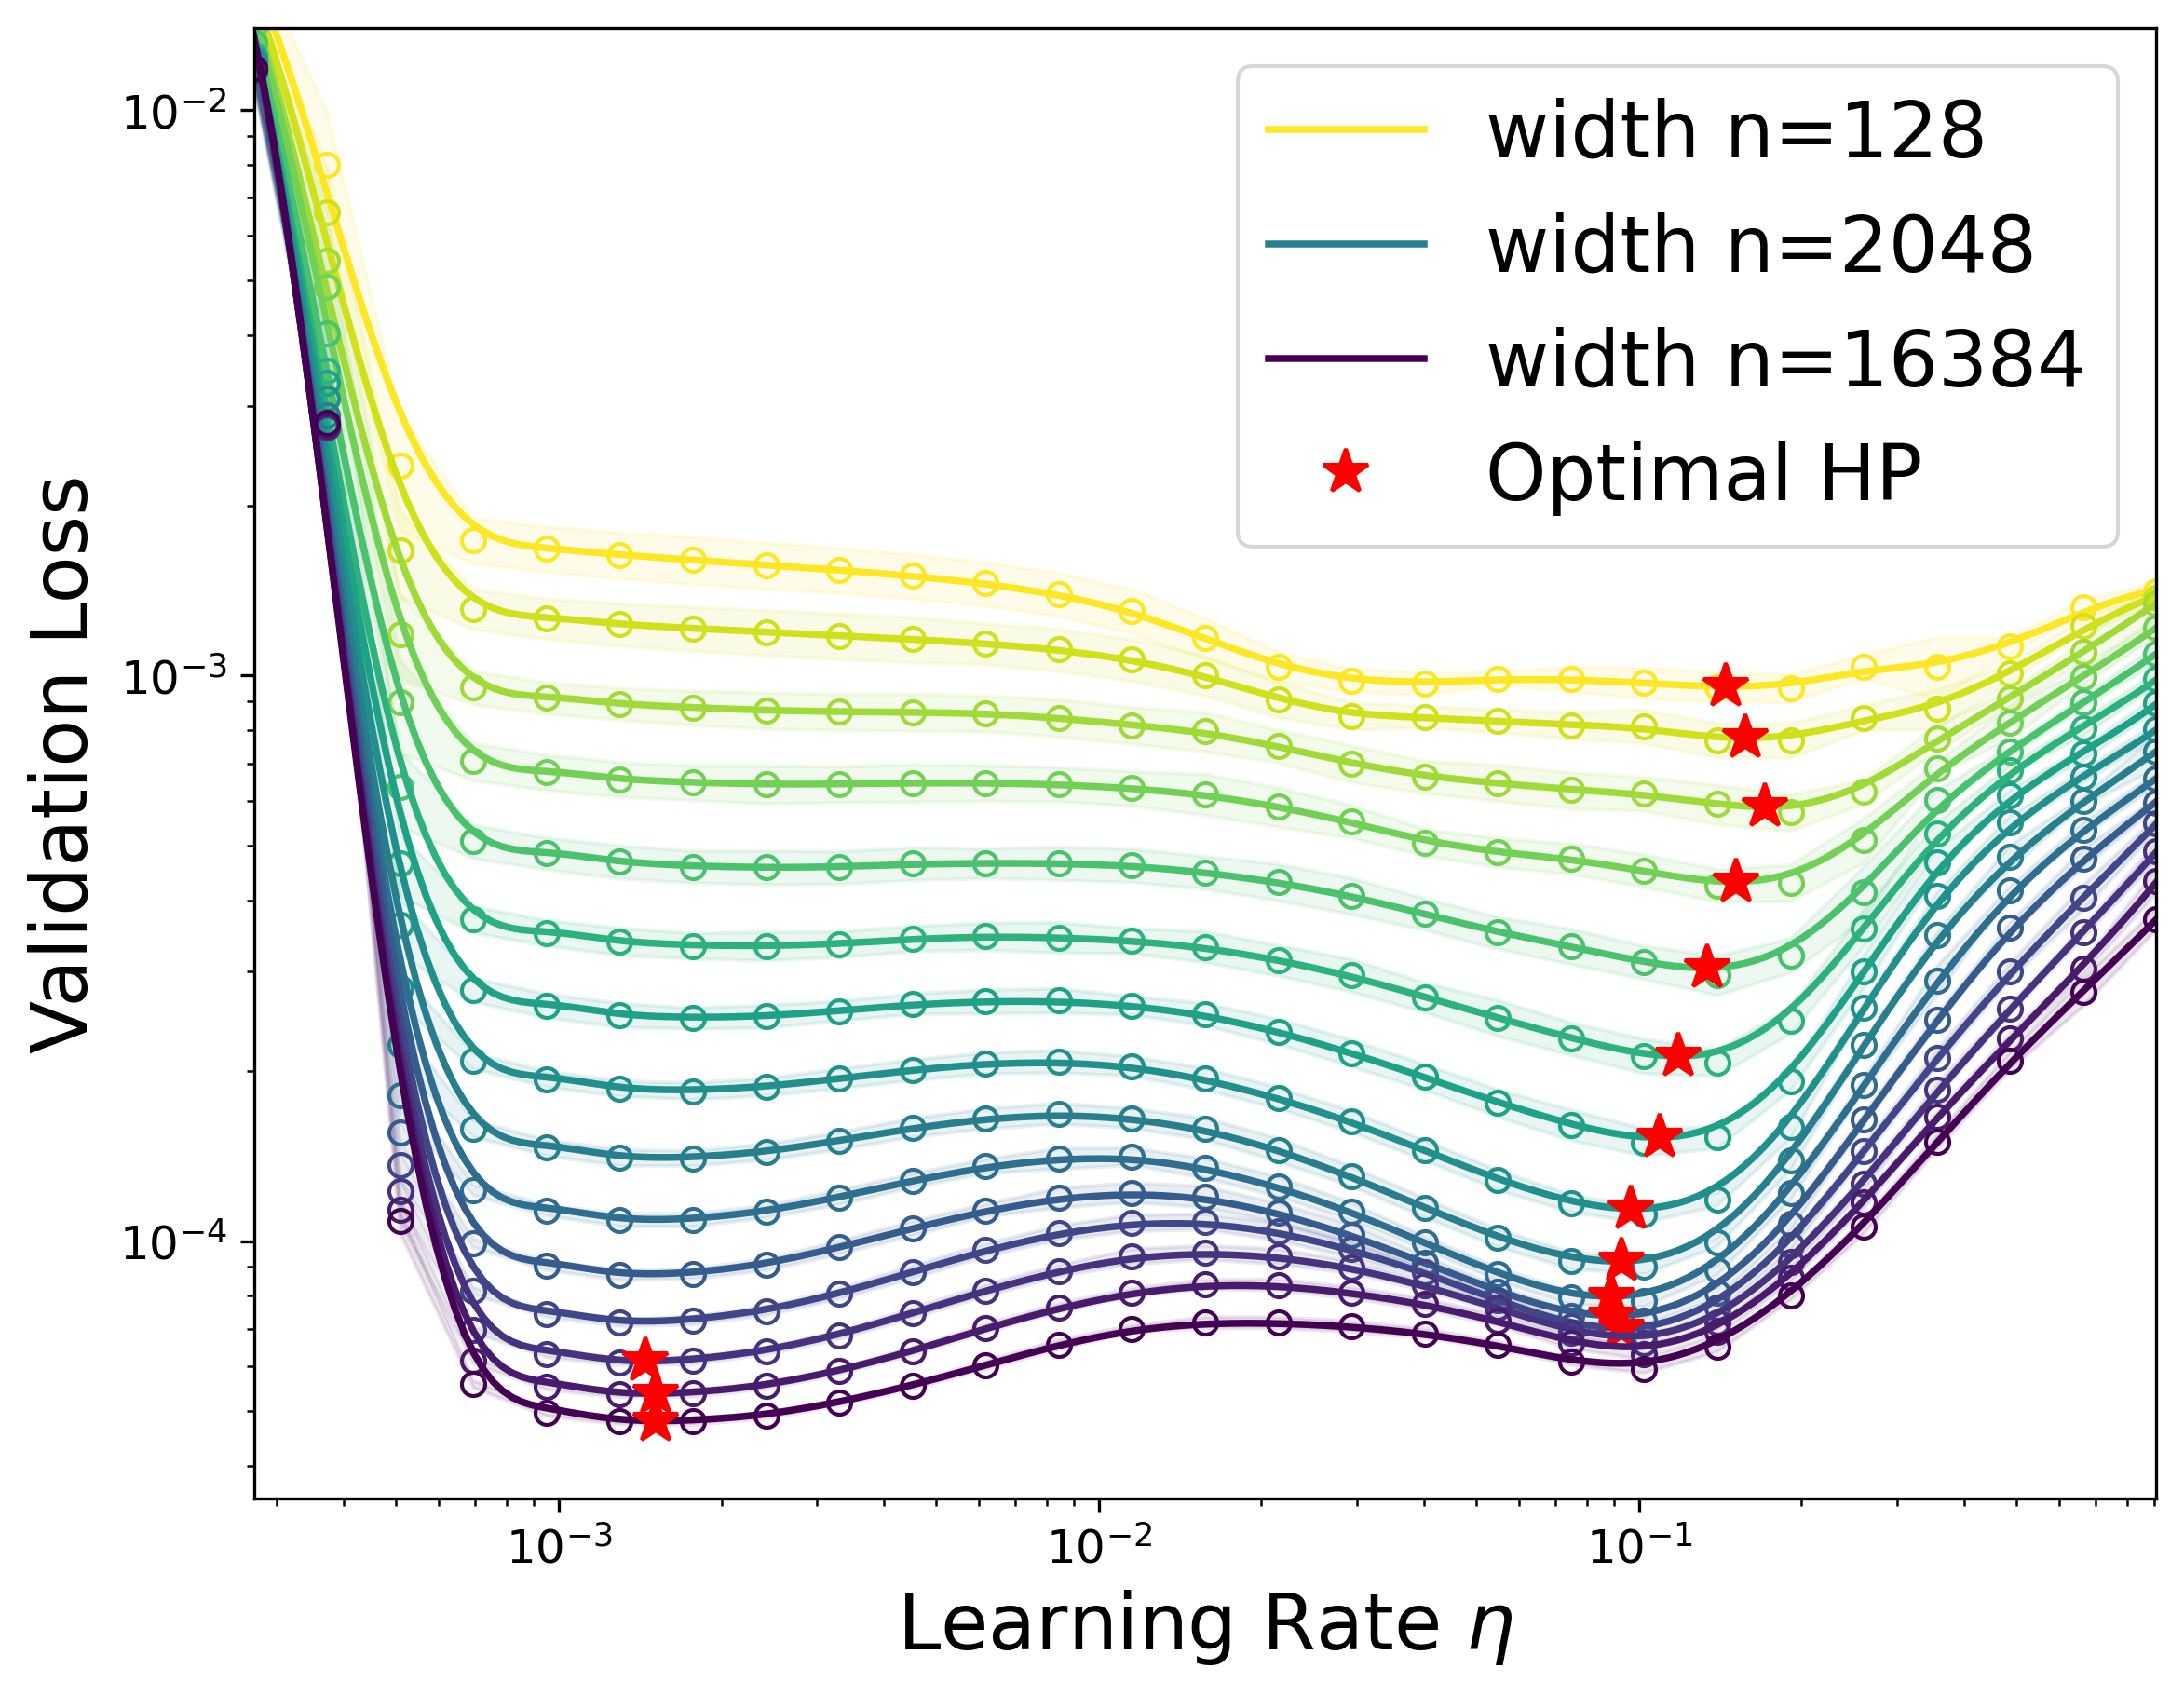
\includegraphics[width=0.42\textwidth,keepaspectratio]{figures/two_layer_ReLU_k_15_d_64_regression_loss_prefactor1.png} 
    \vspace{-6.6mm}
    \caption{\small Learning Gaussian $k$-index model using two-layer ReLU network with $\mu$P. The HP of interest is the Adam learning rate. Experiment details can be found in Appendix~\ref{app:two-layer-relu}. The optimal HP exhibits an abrupt shift at $n=8192$.}
    \label{fig:counter-example}
    \vspace{-6mm}
\end{wrapfigure}

We will say that the parameterization $\bhpexp$ admits \emph{weak transfer} (or simply that ``HP transfer holds'') when the above conditions are satisfied. The rigorous formulation is given in Definition~\ref{def:hp_transfer} (Appendix~\ref{app:background}). We regard this as the ``weakest'' notion of HP transfer, since it concerns only the asymptotic convergence of quantities rather than their convergence rates. Prior work \citep{yang2022tensor, yang2023depth} has argued informally that only ``optimal'' parameterizations can admit weak HP transfer and that $\mu$P is the unique optimal parameterization for general tasks. We formalize the first claim in Theorem \ref{thm:transfer_optimality} and assume that weak transfer holds under $\mu$P. 


Note that weak transfer alone does not imply that transfer under $\mu$P is actually \emph{useful}, as it does not quantify the convergence rates and computational gain over direct tuning. In particular, even though the optimal HP converges to a well-defined limit, if such convergence happens very slowly, then one cannot reliably infer $\bhp^\star(\infty)$ from small-scale proxies --- see Figure~\ref{fig:counter-example} for a numerical example, where the optimal HP up to width $n=8192$ becomes clearly suboptimal for larger-width models.  
In the next section, we will show that stronger conditions on the convergence rates are required for fast and useful HP transfer. 